\documentclass{beamer}
\mode<presentation>
{
  \usetheme{Boadilla}
  \setbeamercovered{transparent}
}
\usepackage[russian]{babel}
\usepackage[utf8]{inputenc}
\usepackage[T2A]{fontenc}
\usepackage{listings}
\setbeamertemplate{navigation symbols}{}
\title[Cloud Haskell]{Cloud Haskell и все все все}
\author{Александр Вершилов}
\setbeamerfont{institute}{size=\normalize}

\begin{document}

\section{Вступление}
\begin{frame}{Вступление}
  План:
  \begin{itemize}
    \item Краткое описание архитектуры \texttt{Cloud-Haskell}
    \item Текущий статус
    \item Расширение Static Pointers
  \end{itemize}
\end{frame}

\begin{frame}{}
  Распределенное программирование покрывает много систем
  \begin{itemize}
    \item от слабосвязанные систем (SOA)
      \begin{itemize}
        \item REST API
        \item HTTP EndPoints
        \item Расширяемые протоколы JSON/XML
      \end{itemize}
    \item до сильно связаных систем
      \begin{itemize}
        \item RPC
        \item протоколы передачи сообщений
        \item фиксированные схемы общения
        \item формат сообщений является внутренним
      \end{itemize}
  \end{itemize}
\end{frame}

\begin{frame}{Что тут может дать Haskell?} \begin{itemize}
    \item Поддержка библиотек (wai,http-client, aeson, cloud haskell, \ldots)
    \item Легкая возможность подключения внешних библиотек (CCI, zmq, \ldots)
    \item Оптимизирующий компилятор
    \item Достаточно мощная система типов
    \item Язык поддерживающий высокоуровневые абстракции
  \end{itemize}
\end{frame}

\begin{frame}{В чем задачи Cloud Haskell}
  \begin{itemize}
    \item Слоган: Erlang в Haskell
    \item Идея: управление кластером "в целом" \\
          (расширение идеи программирования многопроцессорных систем)
    \item Запуск исполняемого файла, который может работать \\
          с распределенными ресурсами как с локальными
    \item Реализуется библиотекой без расширений компилятора (почти)
  \end{itemize}
\end{frame}

\begin{frame}{Модель исполнения}
  \begin{itemize}
    \item Используется Actor model
      \begin{itemize}
        \item явная конкурентность
        \item использование легковесных процессов
        \item наличие только локального состояния
        \item взаимодействие путем обмена сообщениями
      \end{itemize}
    \item Любую программу можно представить в виде Actor модели
    \item Cloud Haskell не единственная Haskell \\
          библиотека использующая модель актёров
  \end{itemize}
\end{frame}

\begin{frame}{Гибкость}
  В основе дизайна Cloud Haskell стояла легкая возможность
  адаптации библиотеки к разным условиям.
  \begin{itemize}
    \item различные реализации транспорта (железо и протоколы) \\
          (TCP, non-IP сети, unix-pipes, shared memory)
    \item различные способы устанавки исполняемых файлы и иницилизировать
          окружения
          (scp/ssh, менеджер задач (azure), API облака, загрузка контейнеров)
    \item различные способы конфигурации исполняемых файлов
          (переменные окружения, параметры запуска, настройки в менеджере)
    \item различные способы поиска узлов в сети
          (динамический поиск в сети, использование master узла, список всех
          известных узлов)
  \end{itemize}
\end{frame}

\begin{frame}{Архитектура}
  \begin{figure}
    \centering
    \def\svgwidth{0.75\columnwidth}
    \input{images//c-h-architecture.pdf_tex}
  \end{figure}
\end{frame}

\begin{frame}{Network Transport - 1}
  \begin{itemize}
    \item API ориентировано на отправку сообщений \\
          \texttt{type Message = [ByteString]}
    \item легковесные однонаправленные каналы
    \item управление свойствами соединения (Reliable/Unriable/Ordered/Unordered)
 \end{itemize}
 \begin{figure}
   
\includegraphics[width= \paperwidth]{images/c-h-n-t.png}
 \end{figure}
\end{frame}

\begin{frame}[fragile]{Network Transport - 2}
  \begin{itemize}
    \item API (упрощенное)
    \begin{itemize}
      \item
\begin{verbatim}
Transport { newEndPoint :: IO EndPoint
          , transportClose :: IO ()
          }
\end{verbatim}
      \item 
\begin{verbatim}
EndPoint { receive :: EndPoint -> IO Event
         , endPointClose :: IO ()
         , address :: EndPointAddress
         , connect :: EndPointAddress -> IO Connection
         }
\end{verbatim}
      \item
\begin{verbatim}
Connection { send :: Message -> IO ()
           , close :: IO ()
           }
\end{verbatim}
    \end{itemize}
  \item Существующие реализации
    \begin{itemize}
      \item TCP (стабильное)
      \item CCI (стабильное)
      \item zeromq (экспериментальное)
      \item in-memory (экспериментальное)
      \item p2p (???)
    \end{itemize}
  \end{itemize}
\end{frame}

\begin{frame}{Distributed Process - 1}
  \begin{itemize}
    \item Процессы (тред Haskell)
    \item Легковесное соедиения для каждой пары общающихся процессов
    \item Message Handler (MH) -- поток распределяющий сообщения, события
    \item Node Controller (NC) -- запуск, связывание процессов, мониторинг, управление реестром
    \item Node Agent (Logger, пользовательские агенты).
  \end{itemize}
\end{frame}

\begin{frame}{distributed-process layer}
 \begin{figure}
   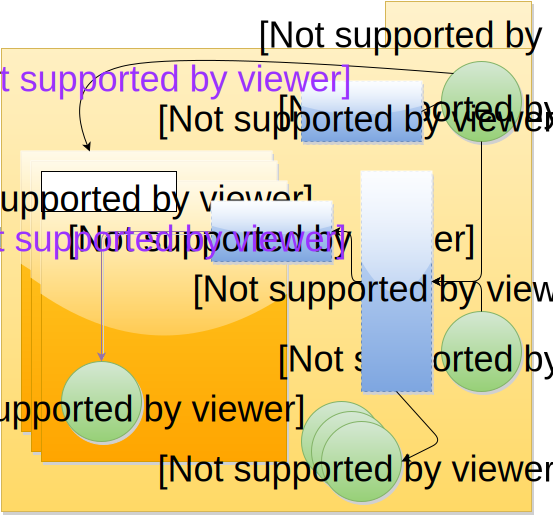
\includegraphics[height=0.85\paperheight]{images/c-h-d-p.png}
 \end{figure}
\end{frame}

\begin{frame}{API}
  \begin{itemize}
    \item управление процессами
    \begin{itemize}
      \item data ProcessId
      \item data Process a
      \item newLocalNode :: Transport $\rightarrow$ IO LocalNode
      \item forkProcess :: LocalNode $\rightarrow$ Process () $\rightarrow$ IO ProcessID
      \item spawn :: NodeId $\rightarrow$ Closure (Process ()) $\rightarrow$ Process ProcessId
      \item spawnLocal :: Process a $\rightarrow$ ProcessId
    \end{itemize}
    \item отправка сообщений
    \begin{itemize}
      \item send :: Serializable a $\Rightarrow$ ProcessId $\rightarrow$ a $\rightarrow$ Process ()
      \item expect :: Serializable a $\Rightarrow$ Process a
    \end{itemize}
  \end{itemize}
\end{frame}

\begin{frame}{Каналы в Cloud Haskell}
  \begin{itemize}
    \item неконтролируемая отправка сообщений может приводить к проблемам разного рода
    \begin{itemize}
      \item возможность memory leak, нужно периодически очищать очередь от неизвестных сообщений
      \item нет проверки системой типов
    \end{itemize}
    \item Каналы
      \begin{itemize}
        \item Позволяют типизировать сообщения
        \item Позволяют не тегировать передаваемые данные
        \item API
    \begin{itemize}
      \item newChan :: Serializable a $\Rightarrow$ Process (SendPort a, ReceivePort a)
      \item (Functor ReceivePort, Applicative ReceivePort, Monad ReceivePort, Serializable SendPort)
      \item sendChan :: Serializable a $\Rightarrow$ SendPort a $\rightarrow$ a $\rightarrow$ Process ()
      \item receiveChan :: Serializable a $\Rightarrow$ ReceivePort a $\rightarrow$ Process a
      \item mergePortsBiased, mergePortsRR
    \end{itemize}
  \end{itemize}
  \end{itemize}
\end{frame}

\begin{frame}{Сериализация и передача функций - 1}
  \begin{itemize}
    \item В haskell в отличии от VM-языков сериализация не является свойством среды
    \item Не все значения могут быть сериализованы
    \item class (Binary a, Typeable a) $\Rightarrow$ Serializable a
    \item С сериализаций функций все сложнее, особенно если в функции есть свободные переменные
    \item spawn :: Closure (Process a) -> Process ProcessId
  \end{itemize}
\end{frame}

\begin{frame}{Сериализация и передача функций - 2}
  \begin{itemize}
    \item Разрешаем сериализацию только "статических функций", нету свободных переменных
            или переменные определены в toplevel.
    \item data Static a
    \item Такие функции можно применять к сериализуемым значением и результат будет сериализуем
    \item data Closure a
\end{itemize}
\end{frame}

\begin{frame}{Сериализация и передача функций - 3}
  \begin{itemize}
    \item Remote Table
      \begin{itemize}
        \item data Closure a = Closure (Static (ByteString -> a)) ByteString
        \item data Static a = Static StaticLabel
        \item data StaticLabel = StaticLabel String | StaticApply StaticLabel StaticLabel
        \item type RemoteTable = Map StaticLabel $\rightarrow$ Dynamic
      \end{itemize}
    \item Проблемы
      \begin{itemize}
        \item Легко приводит к ошибкам
        \item Не типобезопасно
        \item Антимодулярно
      \end{itemize}
  \end{itemize}
\end{frame}

\begin{frame}{Static Pointers - 1}
  {\newblock Towards Haskell in the Cloud, Jeff Epstein, Andrew P. Black, Simon Peyton-Jones}
  \begin{itemize}
    \item расширение \texttt{-XStaticPointers}
    \item конструктор: ключевое слово \alert{static}
    \item выражение должно быть замкнуто
    \item $\Gamma a : A$, static expr $\rightarrow$ StaticPtr a
    \item deRefStaticPtr :: StaticPtr a $\rightarrow$ a
  \end{itemize}
\end{frame}

\begin{frame}{Static Pointers - 2}
  \begin{itemize}
    \item type StaticKey = Fingerprint -- уникальный ключ для выражения под static
    \item data Fingerprint = Fingerprint Word64 Word64
    \item staticKey :: StaticPtr a $\rightarrow$ StaticKey
    \item unsafeLookupStaticPtr :: StaticKey $\rightarrow$ Maybe (StaticPtr a)
    \item в GHC 7.12: \\
      lookupStaticPtr :: StaticKey $\rightarrow$ ($\forall$ a . Typeable a $\Rightarrow$ StaticPtr a $\rightarrow$ b) $\rightarrow$ Maybe (StaticPtr b)
  \end{itemize}
\end{frame}

\begin{frame}{Static Pointers - 3}
  \begin{itemize}
    \item Для каждого вхождения \texttt{static} генерируется top-level выражение и
      \texttt{StaticKey},\texttt{StaticPtr}, \texttt{StaticPtrInfo} (пакет, модуль, внутренее имя, локация в коде)
    \item \texttt{data StaticPtr a = StaticPtr StaticKey StaticPtrInfo a}
    \item \texttt{static StgWord64 key[2]}
    \item \texttt{static void hs\_hpc\_init\_Main(void) \_\_attribute\_\_((constructor));}
    \item при инициализации модуля создается/или дополняется глобальная хеш таблица
      \texttt{StaticKey} $\rightarrow$ \texttt{StaticPtr}
  \end{itemize}
\end{frame}

\begin{frame}[fragile]{Static Closure - 1}
  \begin{itemize}
    \item URI: https://github.com/tweag/distributed-closure
    \item Находится в разработке
    \item 
\begin{verbatim}
data Closure a where
  StaticPtr :: !(StaticPtr a) -> Closure a
  Encoded :: !ByteString -> Closure ByteString
  Ap :: !(Closure (a -> b)) -> !(Closure a) -> Closure b
\end{verbatim}
    \item существуют и другие подходы к сериализации, см \\
    \url{https://ghc.haskell.org/trac/ghc/blog/simonpj/StaticPointers} \\
    \item
    \texttt{Value :: (StaticPtr (ByteString a)) -> ByteString -> Closure a}
  \end{itemize}
\end{frame}

\begin{frame}[fragile]{Static Closure - 2}
  \begin{itemize}
    \item (квази?)-аппликативный функтор
    \item \alert{c}pure :: \alert{Serializable a $\Rightarrow$} a $\rightarrow$ Closure a
    \item $<*>$ :: Closure (a $\rightarrow$ b) $\rightarrow$ Closure a $\rightarrow$ Closure b
    \item closure :: StaticPointer a $\rightarrow$ Closure a
    \item Пример:
\begin{verbatim}
fac :: StaticPtr (Int -> Int)
fac = static (\x -> x * unstatic (fac <*> cpure (x-1)))

fac50on :: NodeId -> Process Int
fac50on = call node (fac <*> pure 50)
\end{verbatim}
  \end{itemize}
\end{frame}

\begin{frame}
  \begin{itemize}
    \item необходимо быть осторожным при вызове кода удаленно
    \item требуется минимальная поддержка среды выполнения
    %\item пока не известно публичных историй успеха при работе в гетерогенных кластерах
    \item C-H предоставляет основу для построения более высокоуровневых систем
    \begin{itemize}
      \item построение data-parallelism 
      \item MapReduce, распределенный NestedDataParallelism, DAG из преобразований (Spark)
    \end{itemize}
  \end{itemize}
\end{frame}


\end{document}
